\documentclass[11pt,a4paper]{article}

% Self-contained source: no external images, fonts, or bibliography files.
% Build: pdflatex -halt-on-error -output-directory=docs docs/project-architecture.tex
% Run the same command a second time to resolve page references.
\usepackage[T1]{fontenc}
\usepackage[utf8]{inputenc}
\usepackage{lmodern}
\usepackage[margin=18mm]{geometry}
\usepackage{microtype}
\usepackage[table]{xcolor}
\usepackage{tikz}
\usetikzlibrary{arrows.meta,positioning,fit,backgrounds,calc}
\usepackage{array,tabularx,booktabs}
\usepackage{enumitem}
\usepackage{fancyhdr}
\usepackage{listings}
\usepackage{hyperref}

\definecolor{ink}{HTML}{17324D}
\definecolor{blue}{HTML}{2563A6}
\definecolor{bluewash}{HTML}{EAF2FB}
\definecolor{green}{HTML}{277563}
\definecolor{greenwash}{HTML}{EAF6F1}
\definecolor{amber}{HTML}{966016}
\definecolor{amberwash}{HTML}{FFF4DF}
\definecolor{muted}{HTML}{536373}
\definecolor{line}{HTML}{CCD6DF}
\definecolor{paper}{HTML}{F5F7FA}

\hypersetup{colorlinks=true,linkcolor=blue,urlcolor=blue,
  pdftitle={Legacy Code Modernization: Architecture Explained},
  pdfauthor={Project architecture documentation}}
\pagestyle{fancy}
\fancyhf{}
\fancyhead[L]{\small\color{muted}Legacy Code Modernization}
\fancyhead[R]{\small\color{muted}Planned architecture}
\fancyfoot[L]{\small\color{muted}Based on the repository's AGENTS.md}
\fancyfoot[R]{\small\thepage}
\setlength{\headheight}{14pt}
\setlength{\parindent}{0pt}
\setlength{\parskip}{7pt}
\setlength{\emergencystretch}{2em}
\setlist[itemize]{leftmargin=*,itemsep=3pt,topsep=4pt}
\renewcommand{\arraystretch}{1.15}
\newcolumntype{Y}{>{\raggedright\arraybackslash}X}
\newcommand{\pageheading}[2]{%
  {\small\color{blue}\sffamily\bfseries #1}\par
  {\LARGE\color{ink}\sffamily\bfseries #2}\par\vspace{3mm}}
\newcommand{\callout}[2]{%
  \par\noindent\colorbox{#1}{%
    \parbox{\dimexpr\linewidth-2\fboxsep\relax}{\strut #2\strut}}\par}
\newcommand{\smalltitle}[1]{\par\medskip{\large\sffamily\bfseries\color{ink}#1}\par}

\tikzset{
  box/.style={draw=blue!65,fill=bluewash,rounded corners=3pt,
    line width=.7pt,align=center,text=ink,font=\small,
    inner sep=7pt,minimum height=13mm},
  service/.style={box,draw=green!65,fill=greenwash},
  guard/.style={box,draw=amber!75,fill=amberwash},
  plain/.style={box,draw=line,fill=paper},
  flow/.style={-{Latex[length=2mm]},draw=blue,line width=.85pt},
  evidence/.style={-{Latex[length=2mm]},draw=green,line width=.85pt},
  control/.style={-{Latex[length=2mm]},draw=muted,dashed,line width=.75pt},
  note/.style={font=\footnotesize,text=muted,align=center},
  boundary/.style={draw=amber,dashed,rounded corners=5pt,line width=.9pt,
    inner sep=5mm}
}
\lstset{basicstyle=\ttfamily\small,backgroundcolor=\color{paper},
  frame=single,rulecolor=\color{line},breaklines=true,
  columns=fullflexible,keepspaces=true,showstringspaces=false}

\begin{document}

\pageheading{01 / THE BIG PICTURE}{Give old software a new engine}

The tool takes a small program written for \textbf{Python 2.7} and produces a
version for \textbf{Python 3.12}. It first records what the old program actually
does, then checks the upgraded version against those records.

\callout{amberwash}{\textbf{Status: design, not an implementation report.}
At authoring time, the repository contains the project instructions in
\texttt{AGENTS.md}; no implementation or checkpoint evidence exists.
All components below are planned. This document records no measured results.}

\begin{center}
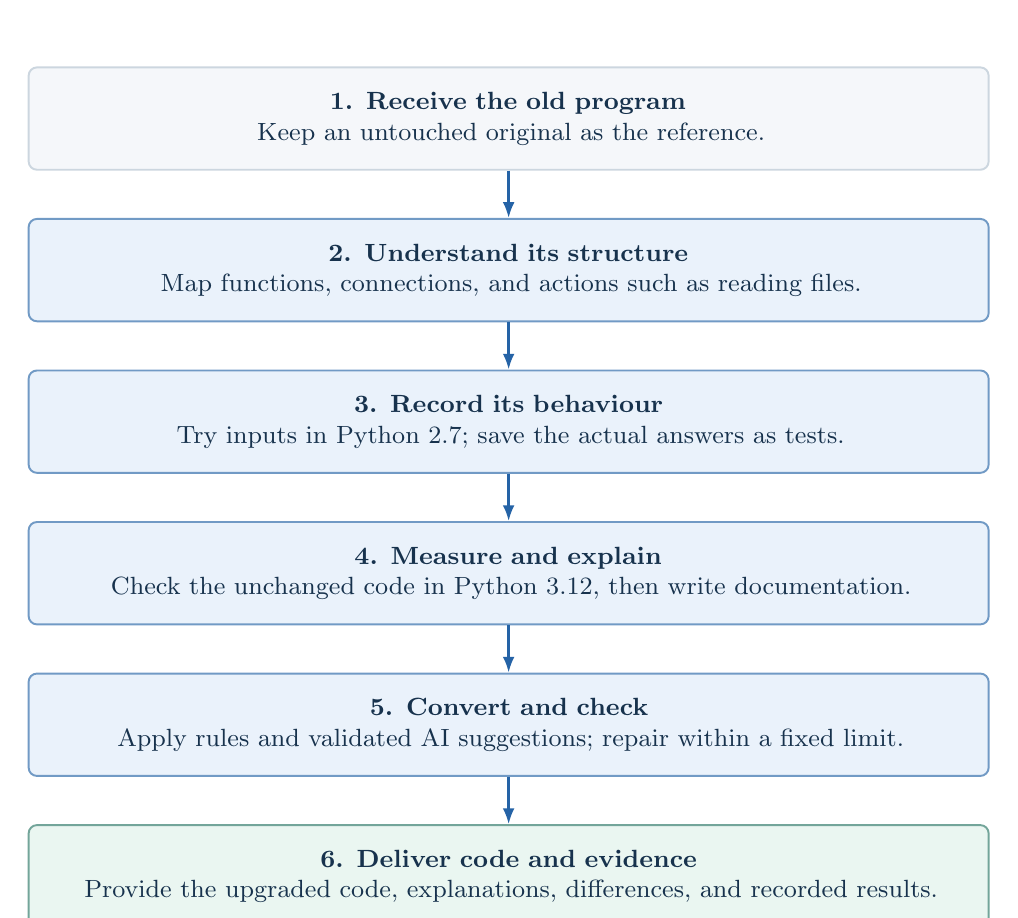
\begin{tikzpicture}
  \node[plain,text width=11.7cm] (input) {\textbf{1. Receive the old program}\\
    Keep an untouched original as the reference.};
  \node[box,text width=11.7cm,below=6mm of input] (map) {\textbf{2. Understand its structure}\\
    Map functions, connections, and actions such as reading files.};
  \node[box,text width=11.7cm,below=6mm of map] (observe) {\textbf{3. Record its behaviour}\\
    Try inputs in Python 2.7; save the actual answers as tests.};
  \node[box,text width=11.7cm,below=6mm of observe] (baseline) {\textbf{4. Measure and explain}\\
    Check the unchanged code in Python 3.12, then write documentation.};
  \node[box,text width=11.7cm,below=6mm of baseline] (upgrade) {\textbf{5. Convert and check}\\
    Apply rules and validated AI suggestions; repair within a fixed limit.};
  \node[service,text width=11.7cm,below=6mm of upgrade] (output) {\textbf{6. Deliver code and evidence}\\
    Provide the upgraded code, explanations, differences, and recorded results.};
  \foreach \from/\to in {input/map,map/observe,observe/baseline,baseline/upgrade,upgrade/output}
    \draw[flow] (\from) -- (\to);
\end{tikzpicture}
\end{center}

\smalltitle{Think of restoring an old machine}
First photograph its parts and measure how it works. Replace the engine, then
repeat the same measurements. Even an odd behaviour must be preserved if it was
present before; suspected old bugs are flagged for people to review.

\textbf{What the checks establish:} whether the recorded behaviours still match.
A passing test suite cannot prove that every possible input behaves identically.

\newpage
\pageheading{02 / SYSTEM MAP}{Who does what?}

The \textbf{orchestrator} is the project manager: ordinary program code decides
the next step, checks its result, and stops when a required check fails. AI is a
specialist it consults, with no authority to choose the workflow.

\begin{center}
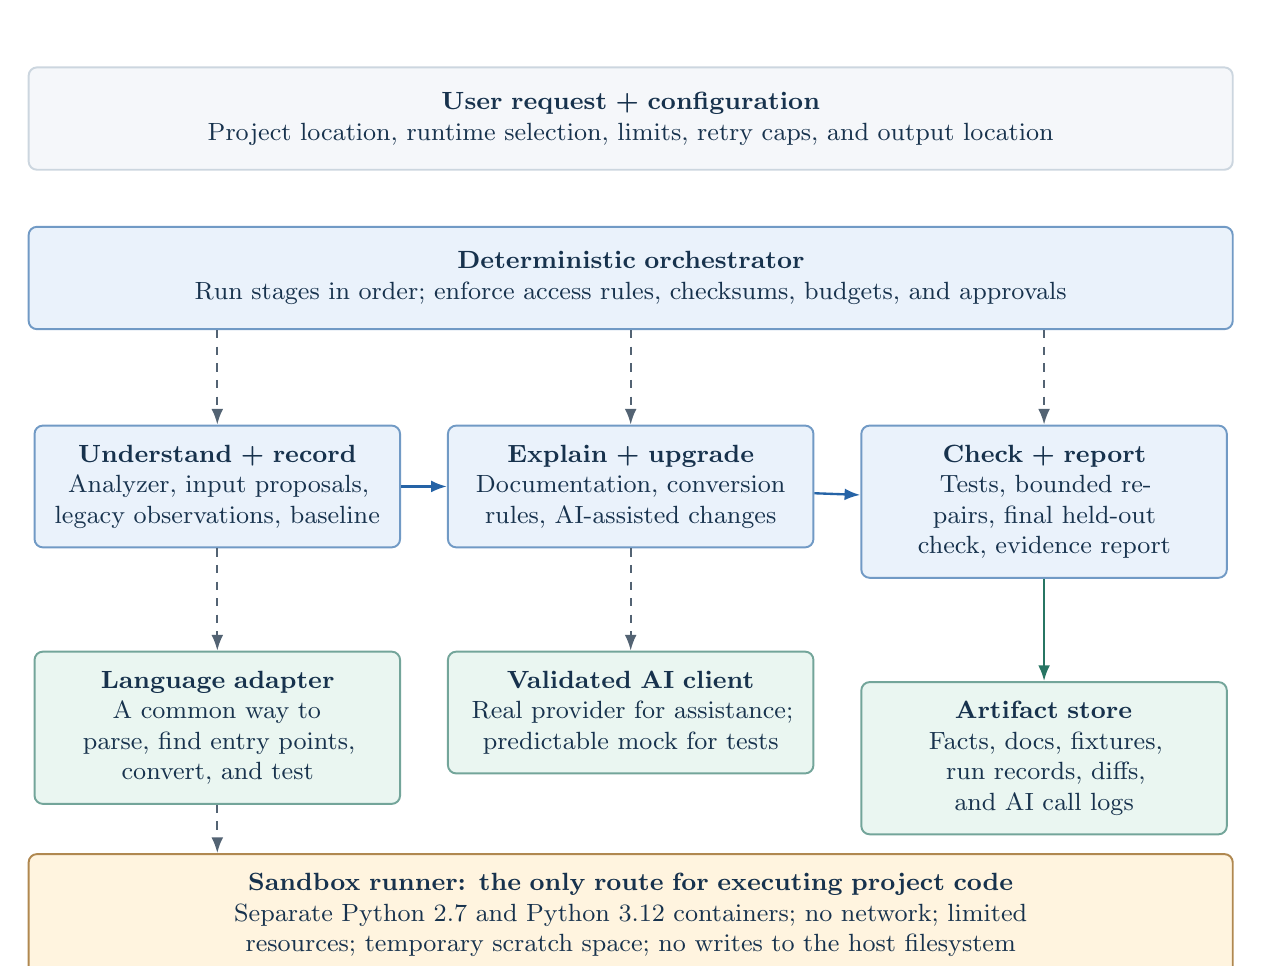
\begin{tikzpicture}
  \node[plain,text width=14.8cm] (request) {\textbf{User request + configuration}\\
    Project location, runtime selection, limits, retry caps, and output location};
  \node[box,text width=14.8cm,below=7mm of request] (manager) {\textbf{Deterministic orchestrator}\\
    Run stages in order; enforce access rules, checksums, budgets, and approvals};
  \node[box,text width=4.15cm,below=12mm of manager,xshift=-5.25cm] (understand)
    {\textbf{Understand + record}\\Analyzer, input proposals, legacy observations, baseline};
  \node[box,text width=4.15cm,below=12mm of manager] (change)
    {\textbf{Explain + upgrade}\\Documentation, conversion rules, AI-assisted changes};
  \node[box,text width=4.15cm,below=12mm of manager,xshift=5.25cm] (verify)
    {\textbf{Check + report}\\Tests, bounded repairs, final held-out check, evidence report};
  \draw[control] (manager.south -| understand.north) -- (understand.north);
  \draw[control] (manager.south) -- (change.north);
  \draw[control] (manager.south -| verify.north) -- (verify.north);
  \draw[flow] (understand) -- (change);
  \draw[flow] (change) -- (verify);

  \node[service,text width=4.15cm,below=13mm of understand] (adapter)
    {\textbf{Language adapter}\\A common way to parse, find entry points, convert, and test};
  \node[service,text width=4.15cm,below=13mm of change] (llm)
    {\textbf{Validated AI client}\\Real provider for assistance; predictable mock for tests};
  \node[service,text width=4.15cm,below=13mm of verify] (store)
    {\textbf{Artifact store}\\Facts, docs, fixtures, run records, diffs, and AI call logs};
  \draw[control] (understand) -- (adapter);
  \draw[control] (change) -- (llm);
  \draw[evidence] (verify) -- (store);

  \node[guard,text width=14.8cm,below=10mm of llm] (sandbox)
    {\textbf{Sandbox runner: the only route for executing project code}\\
    Separate Python 2.7 and Python 3.12 containers; no network; limited resources;
    temporary scratch space; no writes to the host filesystem};
  \draw[control] (adapter.south) -- ++(0,-4mm) -| (sandbox.north -| adapter.south);
\end{tikzpicture}
\end{center}

\textbf{Read the map:} solid blue arrows show stage order; dashed arrows show
control or service use; green arrows show recorded evidence. Support services
are shared across stages; the diagram shows representative connections.

\callout{greenwash}{\textbf{Two different kinds of isolation.}
The sandbox restricts running code. Separately, stage permissions restrict what
documentation, conversion, repair, and AI prompts can read or change.}

\textbf{Scope:} implement the Python 2 adapter only. The interface leaves a place
for Java or PHP later; those implementations are outside the foundation project.

\newpage
\pageheading{03 / COMPONENT GUIDE}{The parts, in everyday language}

\small
\begin{tabularx}{\linewidth}{@{}p{3.2cm}YY@{}}
\toprule
\textbf{Component} & \textbf{Simple explanation} & \textbf{Its responsibility}\\
\midrule
Orchestrator & A manager following a written checklist.
  & Select the next stage; enforce limits; stop or request review when needed.\\
Configuration and logs & The settings sheet and activity diary.
  & Store runtime settings and limits; record structured events and failures.\\
Language adapter & A connector made for one language.
  & Provide parsing, entry-point discovery, conversion, and test execution
    through a common interface.\\
Static analyzer & A mapmaker who studies the program without running it.
  & Extract functions, classes, signatures, comments, imports, approximate
    calls, and markers for effects such as files, network, or randomness.\\
Sandbox runner & A locked workshop for running unfamiliar machinery.
  & Execute code safely; capture answers, errors, printed messages,
    and files created in scratch space.\\
AI client and validators & An adviser whose suggestions must pass inspection.
  & Propose inputs, write explanations, and suggest changes; validate every
    response and log calls, tokens, cost, and failures.\\
Characterization harness & A recorder that learns what the old program does.
  & Run proposed inputs on the original code, save actual outcomes, measure
    coverage, detect unstable tests, and seal a held-out subset.\\
Baseline evaluator & A before-upgrade inspection.
  & Run the unchanged legacy code on both runtimes and classify failures.\\
Documentation generator & A technical writer using the map and observations.
  & Explain functions first, then modules and the package; label AI-written
    text and flag claims that conflict with observed behaviour.\\
Transformer & A mechanic replacing outdated parts.
  & Apply deterministic rules first; use validated AI help for ambiguous
    behaviour; save all source changes as diffs.\\
Verifier and repair loop & An inspector who allows a limited number of fixes.
  & Compare results with frozen expectations, repair source only, enforce
    retry caps, then run the hidden final checks.\\
Artifact store and reporter & A filing cabinet and its evidence-based summary.
  & Preserve the audit trail and generate a report whose numbers can be
    recomputed from recorded runs.\\
\bottomrule
\end{tabularx}
\normalsize

\smalltitle{Why use a Python 2-aware analyzer?}
Old Python syntax cannot always be read by Python 3's built-in parser. Read it
with a Python 2-capable parser or analyze it inside the old container.
Converting first would lose the original structure that this stage must record.

\smalltitle{What is a ``side effect''?}
An action beyond returning an answer: writing a file, contacting a server,
reading an environment setting, using the clock, or changing shared state.
These actions matter because they can make tests unsafe or inconsistent.

\newpage
\pageheading{04 / EVIDENCE FLOW}{Use the same measuring stick}

The AI may suggest questions to ask the old program. \textbf{Only the original
program supplies the expected answers.} Those saved observations are called
fixtures. Tests and fixtures become read-only before source-changing stages.

\begin{center}
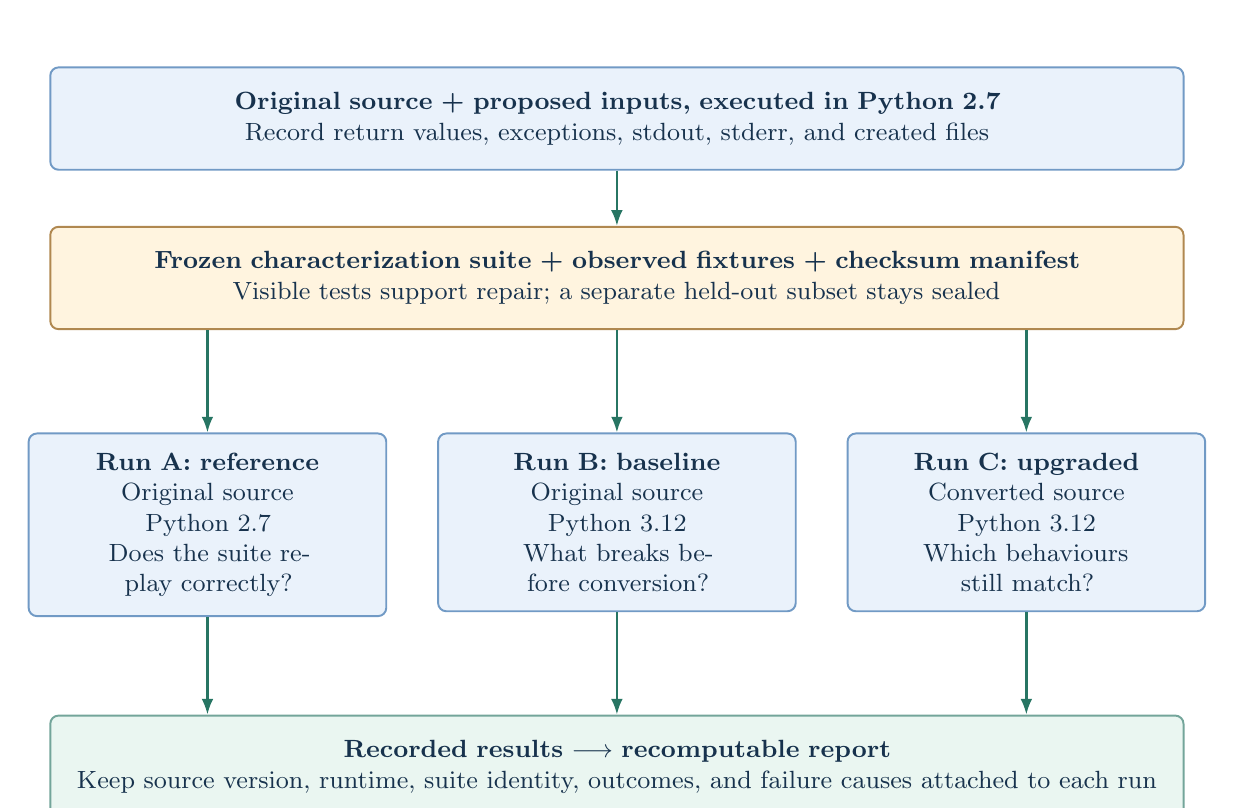
\begin{tikzpicture}
  \node[box,text width=13.9cm] (oracle) {\textbf{Original source + proposed inputs, executed in Python 2.7}\\
    Record return values, exceptions, stdout, stderr, and created files};
  \node[guard,text width=13.9cm,below=7mm of oracle] (frozen)
    {\textbf{Frozen characterization suite + observed fixtures + checksum manifest}\\
    Visible tests support repair; a separate held-out subset stays sealed};
  \draw[evidence] (oracle) -- (frozen);
  \node[box,text width=4.05cm,below=13mm of frozen,xshift=-5.2cm] (a)
    {\textbf{Run A: reference}\\Original source\\Python 2.7\\Does the suite replay correctly?};
  \node[box,text width=4.05cm,below=13mm of frozen] (b)
    {\textbf{Run B: baseline}\\Original source\\Python 3.12\\What breaks before conversion?};
  \node[box,text width=4.05cm,below=13mm of frozen,xshift=5.2cm] (c)
    {\textbf{Run C: upgraded}\\Converted source\\Python 3.12\\Which behaviours still match?};
  \foreach \target in {a,b,c}
    \draw[evidence] (frozen.south -| \target.north) -- (\target.north);
  \node[service,text width=13.9cm,below=13mm of b] (report)
    {\textbf{Recorded results $\longrightarrow$ recomputable report}\\
    Keep source version, runtime, suite identity, outcomes, and failure causes
    attached to each run};
  \foreach \source in {a,b,c}
    \draw[evidence] (\source.south) -- (report.north -| \source.south);
\end{tikzpicture}
\end{center}

\smalltitle{What belongs in the filing cabinet?}
\begin{tabularx}{\linewidth}{@{}p{4.1cm}Y@{}}
\toprule
\textbf{Artifact} & \textbf{Why keep it?}\\
\midrule
AST facts and documentation & Explain structure and preserve the generated descriptions.\\
Fixtures, tests, checksums & Preserve the original answers and detect edits to the exam.\\
Run records and coverage & Back pass rates, failures, and exercised-code measurements.\\
Diffs and repair history & Show exactly what changed, why, and how many repair rounds ran.\\
AI logs and quarantine records & Account for model usage and every excluded unstable test.\\
Sealed held-out tests & Provide an independent final check that repair cannot inspect.\\
\bottomrule
\end{tabularx}

\textbf{Counting rule:} calculate each pass rate from its recorded passed and
total included cases. State the denominator, keep exclusions visible, distinguish
tests blocked by startup or syntax errors, and report held-out results separately.
Do not invent a pass count when code fails to load.

\newpage
\pageheading{05 / EXECUTION BOUNDARY}{A safe workshop for running code}

The runner uses two separate environments: one understands the old program,
the other represents the upgraded destination. Both receive the same execution
restrictions. This applies to original code, converted code, and tests.

\begin{center}
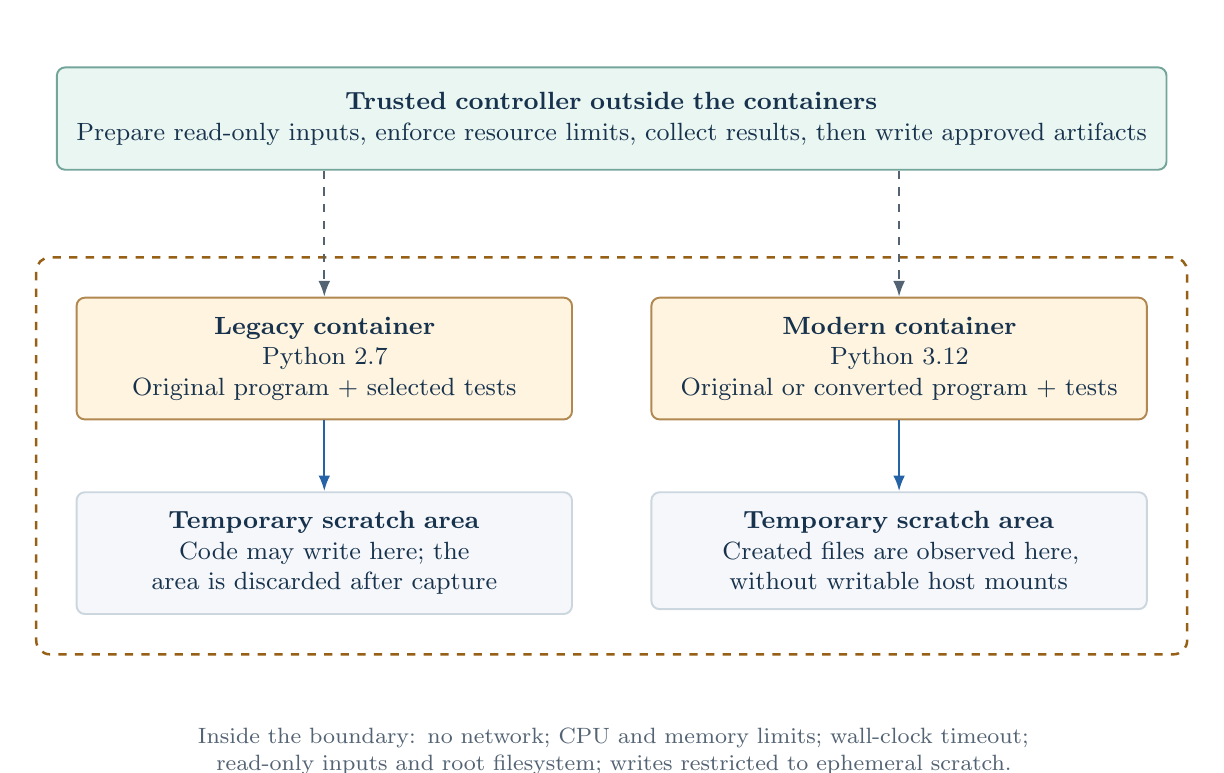
\begin{tikzpicture}
  \node[service,text width=13.6cm] (host) {\textbf{Trusted controller outside the containers}\\
    Prepare read-only inputs, enforce resource limits, collect results,
    then write approved artifacts};
  \node[guard,text width=5.8cm,below=16mm of host,xshift=-3.65cm] (old)
    {\textbf{Legacy container}\\Python 2.7\\Original program + selected tests};
  \node[guard,text width=5.8cm,below=16mm of host,xshift=3.65cm] (modern)
    {\textbf{Modern container}\\Python 3.12\\Original or converted program + tests};
  \node[plain,text width=5.8cm,below=9mm of old] (oldscratch)
    {\textbf{Temporary scratch area}\\Code may write here; the area is discarded after capture};
  \node[plain,text width=5.8cm,below=9mm of modern] (newscratch)
    {\textbf{Temporary scratch area}\\Created files are observed here, without writable host mounts};
  \draw[control] (host.south -| old.north) -- (old.north);
  \draw[control] (host.south -| modern.north) -- (modern.north);
  \draw[flow] (old) -- (oldscratch);
  \draw[flow] (modern) -- (newscratch);
  \begin{scope}[on background layer]
    \node[boundary,fit=(old)(modern)(oldscratch)(newscratch)] (isolated) {};
  \end{scope}
  \node[note,below=8mm of isolated,text width=14.6cm] {
    Inside the boundary: no network; CPU and memory limits; wall-clock timeout;\\
    read-only inputs and root filesystem; writes restricted to ephemeral scratch.};
\end{tikzpicture}
\end{center}

\smalltitle{How results leave the workshop}
The trusted controller captures output and copies approved scratch artifacts out
after execution. The program inside the container never receives permission to
write directly into the host's artifact store. Capture paths and file types must
be checked so a generated link cannot redirect collection outside scratch.

\smalltitle{The AI connection is outside this boundary}
The real AI client may need a provider network connection. It runs in the
trusted control layer, not inside either execution container. API keys stay
outside project code and are excluded from prompts and logs. The mock client
provides predictable responses for tests without an external service.

\callout{amberwash}{\textbf{Isolation requires evidence.}
Checkpoint CP3 must demonstrate that network access fails, runaway execution is
killed, excessive memory use is stopped, outside-scratch writes are prevented or
discarded, and deterministic runs capture the same output twice.}

\newpage
\pageheading{06 / AI AND REPAIR}{An adviser with a checked work order}

Every AI task has a versioned prompt, an expected response structure, a timeout,
and a retry cap. A schema is simply a checklist for the response's fields and
types. Parsing, compilation, and execution checks are added where appropriate.

\begin{center}
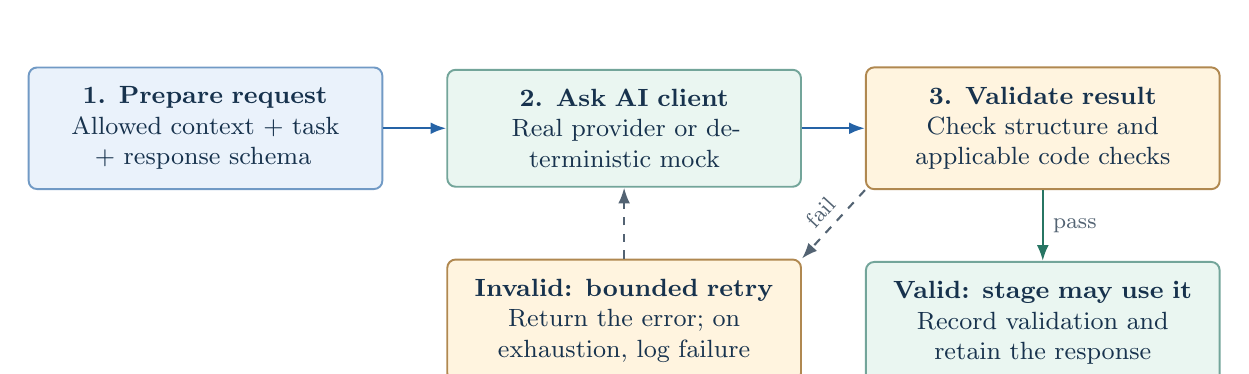
\begin{tikzpicture}
  \node[box,text width=4.0cm] (prompt) {\textbf{1. Prepare request}\\Allowed context + task + response schema};
  \node[service,text width=4.0cm,right=8mm of prompt] (ai) {\textbf{2. Ask AI client}\\Real provider or deterministic mock};
  \node[guard,text width=4.0cm,right=8mm of ai] (validate) {\textbf{3. Validate result}\\Check structure and applicable code checks};
  \draw[flow] (prompt) -- (ai);
  \draw[flow] (ai) -- (validate);
  \node[service,text width=4.0cm,below=9mm of validate] (accept)
    {\textbf{Valid: stage may use it}\\Record validation and retain the response};
  \node[guard,text width=4.0cm,below=9mm of ai] (retry)
    {\textbf{Invalid: bounded retry}\\Return the error; on exhaustion, log failure};
  \draw[evidence] (validate) -- node[right,note]{pass} (accept);
  \draw[control] (validate.south west) -- node[above,sloped,note]{fail} (retry.north east);
  \draw[control] (retry) -- (ai);
\end{tikzpicture}
\end{center}

\textbf{Per-call record:} prompt, response, model, token counts, validation result,
and accounted cost. Provider timeouts and rate limits receive bounded handling;
cost and tokens are summarized per run.

\smalltitle{The repair loop}
\begin{center}
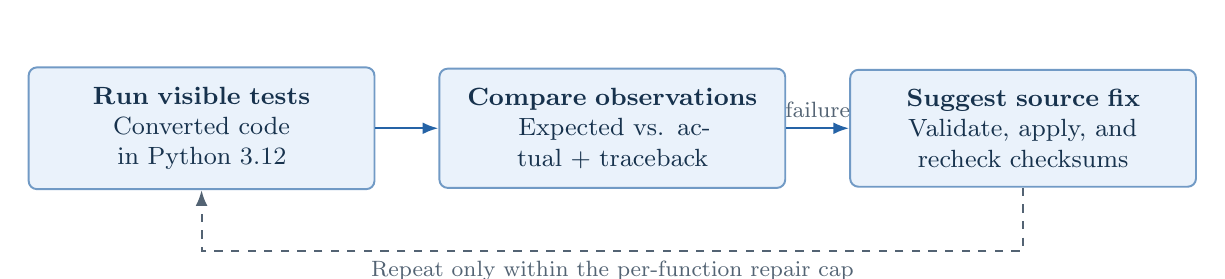
\begin{tikzpicture}
  \node[box,text width=3.9cm] (test) {\textbf{Run visible tests}\\Converted code in Python 3.12};
  \node[box,text width=3.9cm,right=8mm of test] (compare)
    {\textbf{Compare observations}\\Expected vs. actual + traceback};
  \node[box,text width=3.9cm,right=8mm of compare] (repair)
    {\textbf{Suggest source fix}\\Validate, apply, and recheck checksums};
  \draw[flow] (test) -- (compare);
  \draw[flow] (compare) -- node[above,note]{failure} (repair);
  \draw[control] (repair.south) -- ++(0,-8mm) -|
    node[pos=.25,below,note]{Repeat only within the per-function repair cap} (test.south);
\end{tikzpicture}
\end{center}

If visible tests pass, or the repair budget is exhausted, freeze repairs and run
the held-out set as the final check. Unresolved failures are reported as
\textbf{needs human review}. Held-out inputs, expected answers, and detailed
outcomes never feed back into the repair stage or AI context.

\callout{greenwash}{\textbf{Protect the exam.}
Source-editing stages cannot write tests or fixtures. Compare their checksums
before and after documentation, conversion, and repair; a mismatch fails the
stage. Keep the held-out subset in a separate restricted area, accessible only
to its sealing and final-evaluation steps.}

\textbf{Honest results:} review diffs for fixture-specific branches, swallowed
exceptions, or weakened comparisons. Document any normalization rule and apply
it equally to both runtimes. Log every quarantined test. Preserve suspected
legacy bugs. Unexpectedly perfect results trigger a test-strength and leakage
investigation before acceptance.

\newpage
\pageheading{07 / DELIVERY ROADMAP}{Build and approve one checkpoint at a time}

These checkpoints describe implementation order. They are distinct from the
stages executed for an individual project. This architecture document does not
implement, complete, or approve any checkpoint.

\small
\begin{tabularx}{\linewidth}{@{}p{1.0cm}p{3.4cm}Y@{}}
\toprule
\textbf{Step} & \textbf{Build} & \textbf{Evidence required before moving on}\\
\midrule
CP0 & Foundation and environments & Both runtime versions demonstrated; configuration,
logging, mock AI client, and one command for all tests.\\
CP1 & Evaluation corpus & 4--6 licensed or original Python 2 projects; hazard coverage
matrix; all run in Python 2.7; a hand-checkable golden project.
\textbf{Human approval required.}\\
CP2 & Static analyzer & Every corpus file parses; validated fact schema;
tests for each fact type; no AI in analysis.\\
CP3 & Sandbox runner & Isolation and resource limits demonstrated;
structured results; repeatable deterministic output.\\
CP4 & AI layer & Real provider, versioned prompts, schemas, bounded retries,
call logs, timeouts, rate-limit handling, and usage accounting.\\
CP5 & Characterization tests & Repeated legacy replay passes; stated coverage target;
quarantine policy and report; mutation checks meet a stated minimum;
held-out subset sealed.\\
CP6 & Baseline measurement & Original code measured in both runtimes; failure
causes recorded. \textbf{Human approval required.}\\
CP7 & Generated documentation & Functions/classes documented or justified;
module and package summaries; claims cross-checked; tests unchanged.\\
CP8 & Transformation & Rules first, AI for semantic questions; modern compile
and import checks; saved diffs; checksum proof; AI changes explained.\\
CP9 & Verification and repair & Bounded repair rounds; checksum proof; held-out
results reported separately; anti-gaming review recorded.\\
CP10 & Evidence-based report & Three pass rates, coverage, exclusions, held-out
results, diffs, repairs, usage, unresolved issues, and docs;
all numbers recomputable from runs.\\
CP11 & Reproducible hand-off & One-command clean-checkout pipeline across the corpus;
repeat run; README and golden-project demo.
\textbf{Human approval required.}\\
CP12 & Optional dependency report & Only after CP11 approval: assess compatible
packages, trial-install in the modern container, report breakage;
recommend changes without applying them.\\
\bottomrule
\end{tabularx}
\normalsize

\smalltitle{The trial collection must exercise real migration hazards}
Include print statements, old exception syntax, dictionary iteration, integer
division, bytes and Unicode, \texttt{map/filter/zip}, comparison-function sorting,
relative imports, file I/O, and time or randomness.

\textbf{Progress ledger:} record each checkpoint's status, date, exact evidence
commands and outputs, artifact paths, gaps, and decisions in
\texttt{PROGRESS.md}. No checkpoint passes on appearance alone.

\newpage
\pageheading{08 / WALK-THROUGH}{One tiny example ties it together}

\callout{amberwash}{\textbf{Illustration only.}
The example below explains the intended process. It is not a recorded run,
corpus project, fixture, or claimed checkpoint result.}

Suppose the original program divides two integers:
\begin{lstlisting}[language=Python]
# Original Python 2.7 source
def share(total, people):
    return total / people
\end{lstlisting}

\begin{enumerate}[leftmargin=*,itemsep=5pt]
  \item \textbf{Map it.} The analyzer records a function called \texttt{share}
    with two inputs and a division expression.
  \item \textbf{Ask it questions.} AI proposes inputs such as \texttt{(5, 2)},
    \texttt{(0, 2)}, and \texttt{(5, 0)}. The legacy sandbox determines the
    answers, their types, and any exceptions; AI does not supply them.
  \item \textbf{Save the answers.} The harness freezes actual observations in
    fixtures. For ordinary integer inputs, Python 2 integer division is a
    migration hazard: \texttt{5 / 2} yields the integer \texttt{2}, whereas
    Python 3's \texttt{/} yields \texttt{2.5}.
  \item \textbf{Measure before changing anything.} Running the original source
    in Python 3.12 exposes the difference. That result belongs in the baseline.
  \item \textbf{Propose a compatible change.} For a function established to
    take integers, \texttt{total // people} is a candidate. The tool must still
    check the recorded inputs and types; blindly changing every division could
    break functions that also accept floating-point inputs.
  \item \textbf{Repeat the checks.} Re-run frozen tests, respect the repair cap,
    perform the held-out evaluation, and report observed results. If exception
    details differ, do not silently ignore them to manufacture a pass.
\end{enumerate}

\smalltitle{What the user receives at the end}
An upgraded codebase; tagged machine-written docstrings and architecture
summaries; source diffs; before-and-after run records; coverage and exclusions;
separate held-out results; repair counts; AI token and cost totals; unresolved
failures and suspected legacy bugs. Every reported number links back to evidence.

\smalltitle{A small glossary}
\begin{tabularx}{\linewidth}{@{}p{3.0cm}Y@{}}
\toprule
\textbf{Term} & \textbf{Everyday meaning}\\
\midrule
AST & A structured map of the code, like a sentence split into its parts.\\
Fixture & A saved observation used as an expected answer in a later check.\\
Checksum & A digital fingerprint used to detect whether a file changed.\\
Coverage & How much of the program the tests exercised; not a correctness guarantee.\\
Mutation check & Deliberately break a disposable copy and see whether tests notice.\\
Held-out tests & A sealed final exam the repair process cannot study.\\
\bottomrule
\end{tabularx}

\newpage
\pageheading{09 / READING AND BUILDING}{Use this document}

\smalltitle{Choose a route through the diagrams}
\begin{tabularx}{\linewidth}{@{}p{4.3cm}Y@{}}
\toprule
\textbf{What you want to understand} & \textbf{Where to look}\\
\midrule
The purpose in one minute & Page 1: the six-step journey.\\
The system's main pieces & Pages 2--3: the system map and component guide.\\
Why the results are credible & Page 4: reference, baseline, and upgraded runs.\\
Where unfamiliar code runs & Page 5: isolated runtime environments.\\
How AI is controlled & Page 6: validation and bounded repair.\\
How development proceeds & Page 7: checkpoints and approval gates.\\
A concrete example & Page 8: division behaviour before and after conversion.\\
\bottomrule
\end{tabularx}

\smalltitle{Compile the LaTeX source}
This file uses standard LaTeX packages, including TikZ for vector diagrams.
It needs no external images or bibliography. With a LaTeX distribution installed,
run these commands from the repository root:

\begin{lstlisting}[language=bash]
pdflatex -halt-on-error -output-directory=docs docs/project-architecture.tex
pdflatex -halt-on-error -output-directory=docs docs/project-architecture.tex
\end{lstlisting}

The expected output is \texttt{docs/project-architecture.pdf}. Alternatively,
upload the \texttt{.tex} file to a LaTeX editor such as Overleaf and use pdfLaTeX.

\smalltitle{What this design commits to}
\begin{itemize}
  \item The original program is the source of truth for test expectations.
  \item Ordinary code controls the workflow; AI suggestions are validated.
  \item Execution is isolated; source-changing stages cannot change the tests.
  \item Held-out tests remain outside repair access and repair prompts.
  \item All pass rates and usage totals must come from saved run records.
  \item Development follows CP0--CP11 with approval at the specified gates.
\end{itemize}

\smalltitle{What is still a design choice}
The exact Python 2 parser, provider SDK, storage format, conversion tool,
coverage mechanism, and operating-system enforcement details are not selected
by this diagram. Each must satisfy its checkpoint and be justified in the
progress ledger. A workspace directory or a small database may serve as the
artifact store; neither is asserted to exist today.

\callout{bluewash}{\textbf{Source of requirements:} the repository's
\texttt{AGENTS.md}, read on 18 November 2026. This is a human-facing design
overview of the modernization tool. It is separate from the code documentation
that the future tool will generate for each input project at CP7.}

\end{document}
